Tutte le misure di flusso passano attraverso la conoscenza e lo studio dettagliato dell'efficienza dei singoli detector che costituiscono il nostro apparato. Tale studio sarà effettuato a terra presso i laboratori dell'INFN come operazione preliminare al volo, presumibilmente nelle settimane precedenti al lancio. 

La rivelazione della componente carica avviene attraverso due diversi apparati: due sistemi basati su scintillatori e una \emph{micromegas}. Entrambi i detector vengono sviluppati appositamente e gentilmente finanziati dall'INFN. 
\subsection{Scintillatore}
La prima classe di detector sfrutta il \emph{meccanismo di scintillazione} per rivelare le particelle cariche che attraversano un materiale plastico emettendo fotoni raccolti da due SiPM (Silicon PhotoMultiplier) incollati sulle pareti laterali. In particolare, i SiPM utilizzati saranno del tipo NUV (sensibili ultravioletto) della FBK\footnote{https://advansid.com/technology/silicon-photomultipliers}.
Questo sistema scintillatore--SiPM viene letto da un'elettronica di front-end essenzialmente suddivisa in due parti: PCB (che comprende l’amplificatore e il comparatore, oltre che il circuito di alimentazione dei SiPM) e CPU (XLR8 di Alorium con FPGA). Tale apparato è già stato assemblato come mostrato in Figura \ref{Telescopio}.
\begin{figure}
\centering
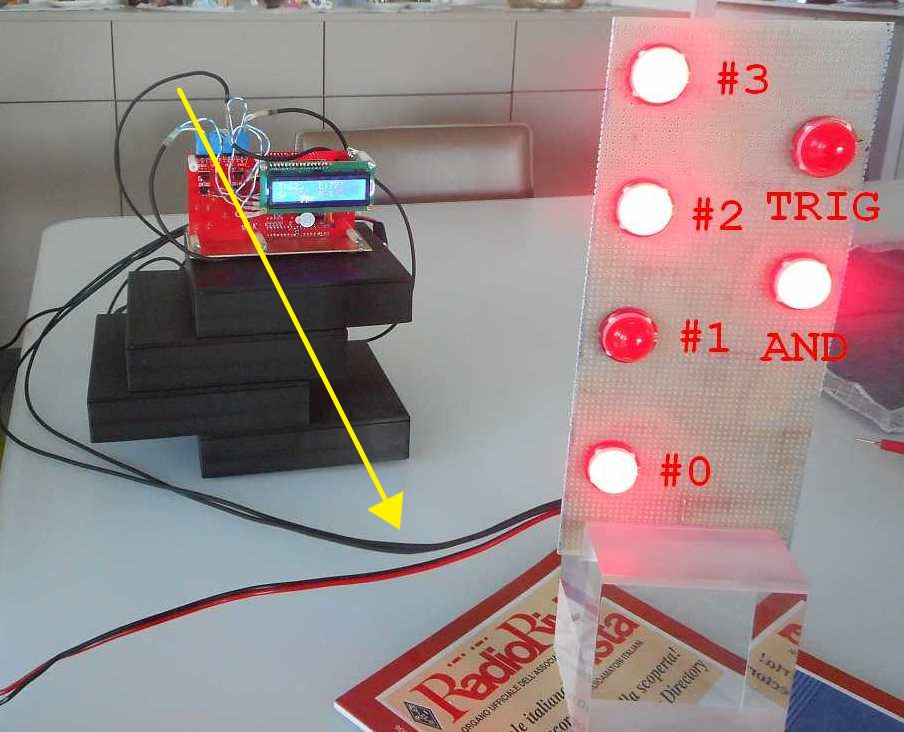
\includegraphics[width=0.35\textwidth]{TRIGGER and(3-0)_event 3-2-0.jpg}
\caption{Test di funzionamento dell'apparato scintillatore.}
\label{Telescopio}

\end{figure}

\subsection{Micromegas}
La micromegas (micro-mesh gaseous structure, MM) è un contatore a valanga a facce piane parallele che consiste in regione di deriva ($\sim 5\,\text{mm}$) e di una moltiplicativa posta tra la micromesh e gli elettrodi di read-out ($\sim 128\,\upmu\text{m} $). 
Quando una particella carica attraversa il detector produce elettroni di ionizzazione nella regione di deriva/conversione, che successivamente si spostano verso la zona moltiplicativa attraverso i buchi nella griglia della mesh, dove vengono amplificati. 

\begin{figure}[!h]
    \centering
    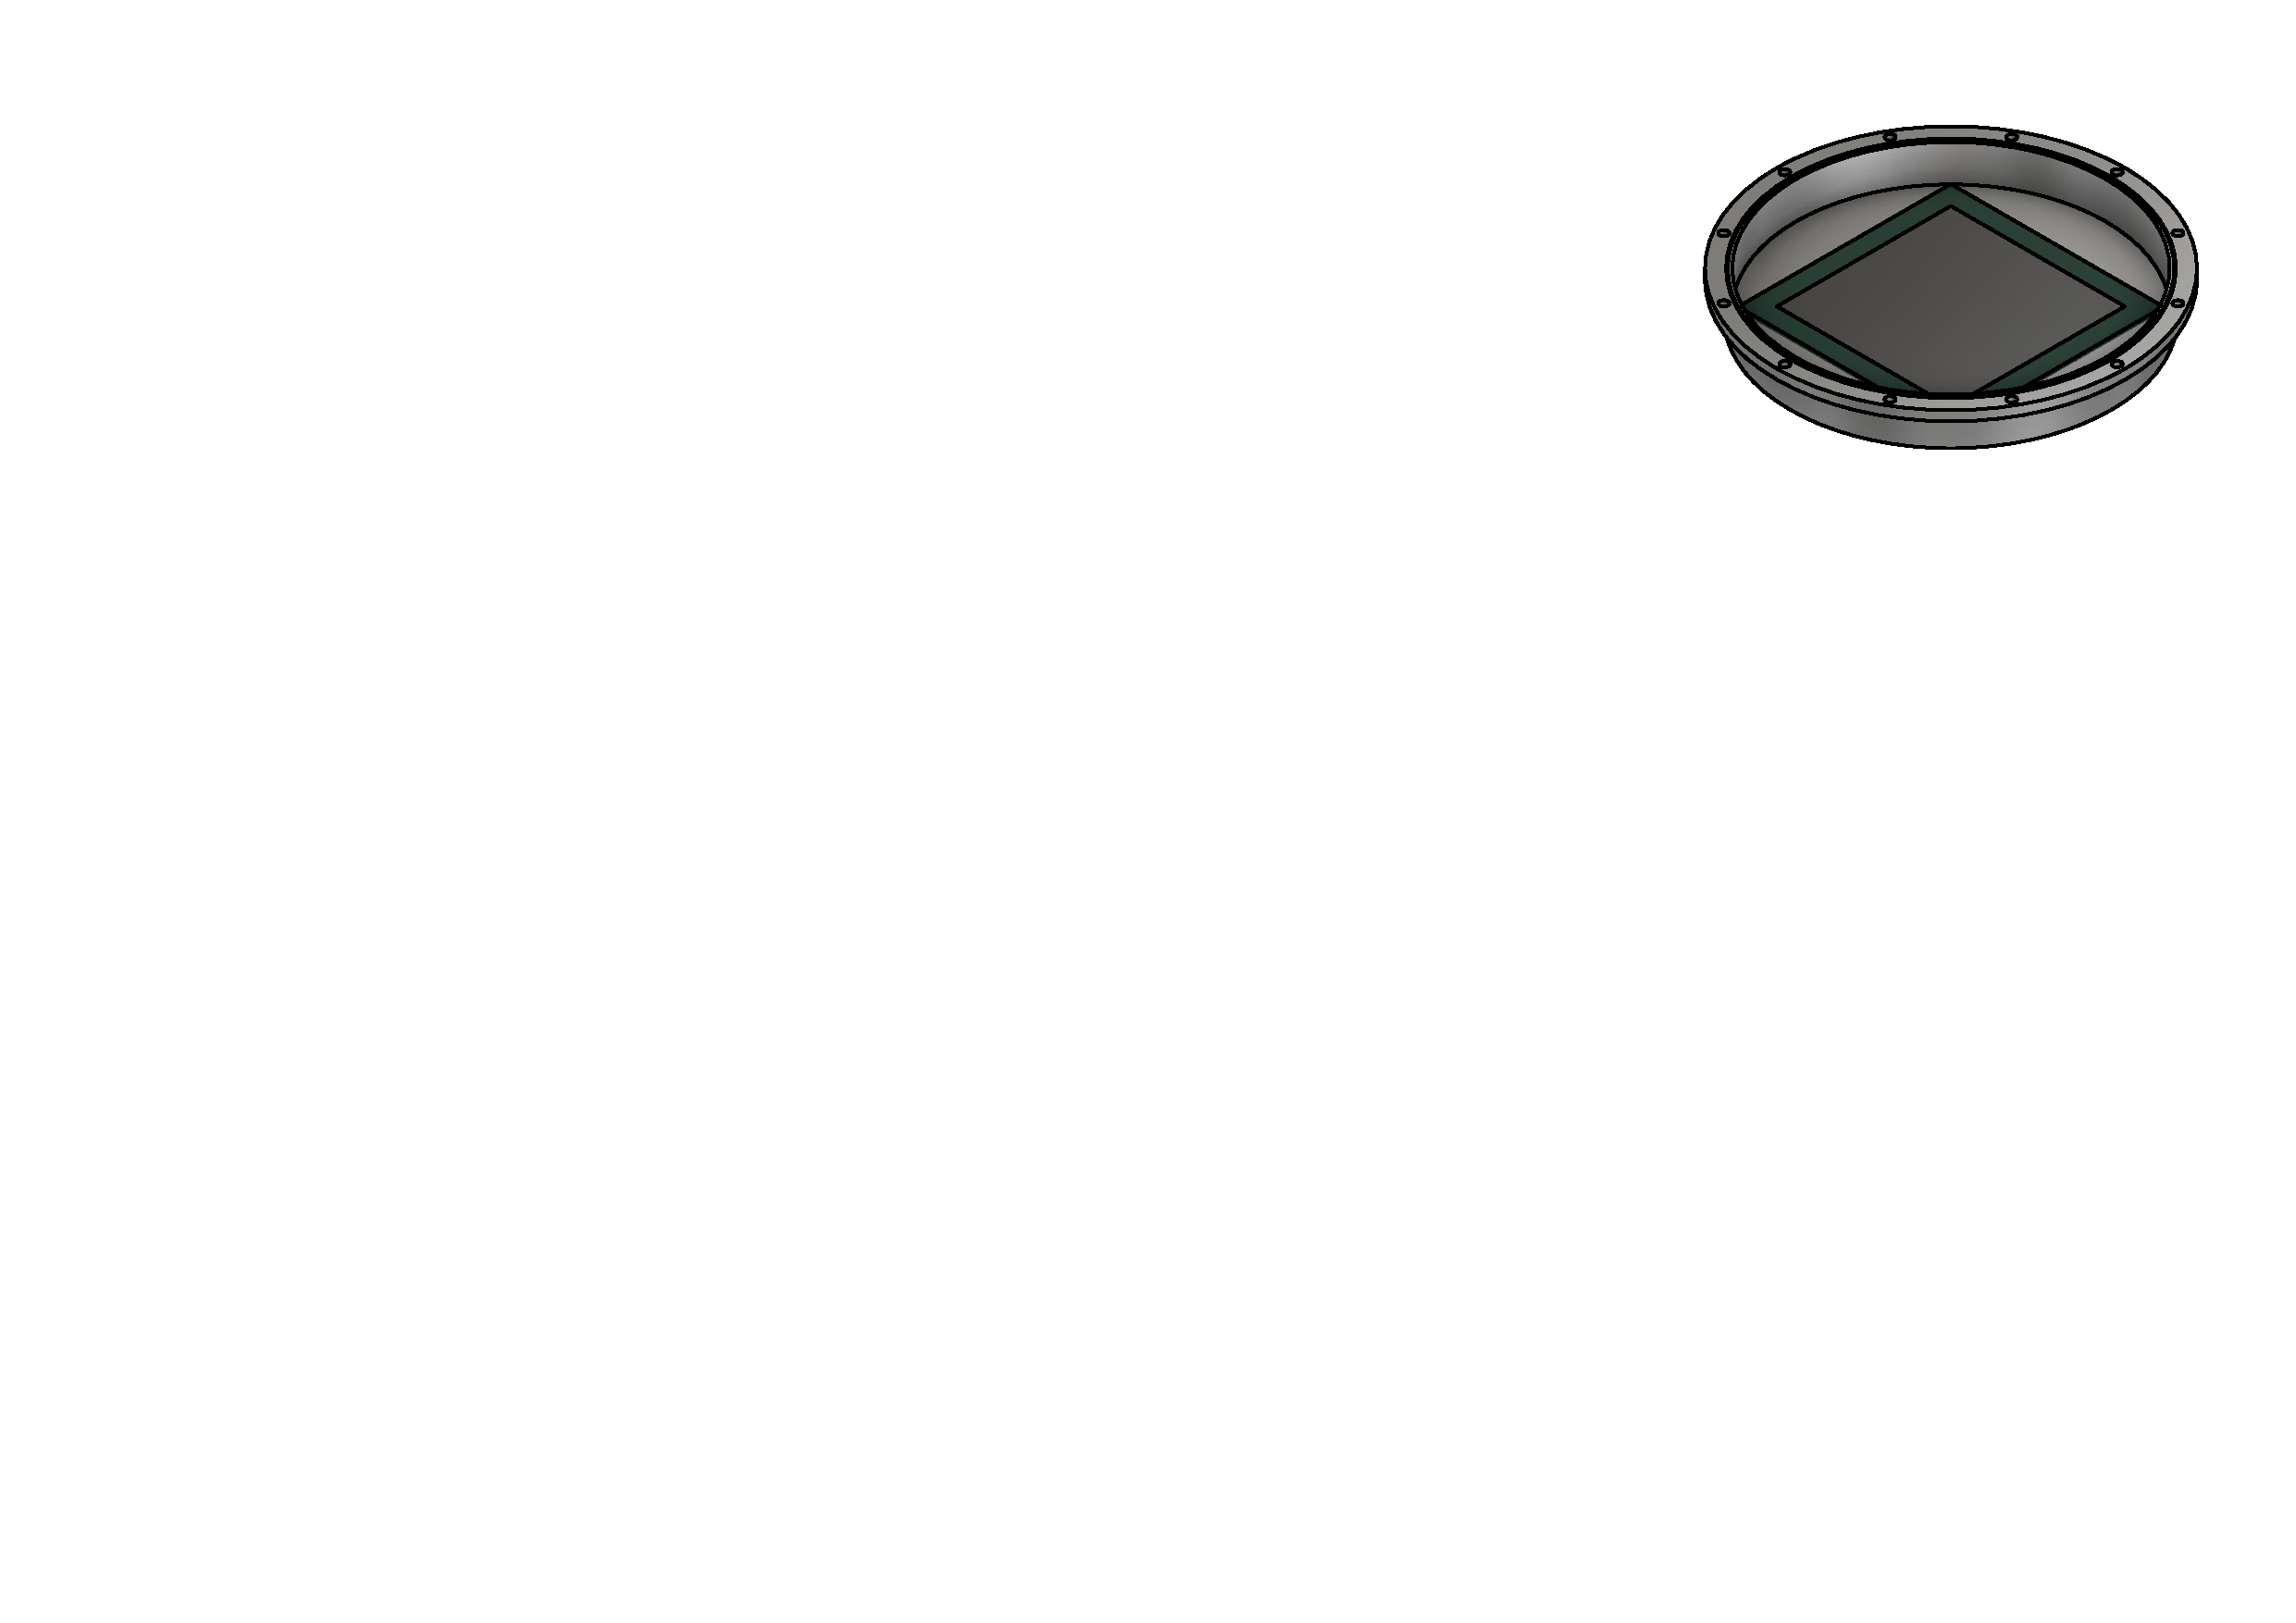
\includegraphics[width=0.4\textwidth]{Micromegas_Disegno.pdf}
    \caption{Proiezione della micromegas e del supporto appositamente progettate per il nostro esperimento.}
    \label{Micromegas_Disegno}
\end{figure}

La micromegas che si implementerà è unica nel suo genere perché ottimizzata anche per la rivelazione degli ENA (atomi neutri di bassa energia) che vengono ionizzati a seguito dell'attraversamento di un foglio di carbonio posto sulla finestra di rivelazione della MM. 
Viste le dimensioni e i pesi non sarà possibile equipaggiarla con un read-out standard, ma sarà letto soltanto il segnale della mesh, corrispondente all’OR di tutte le strip e questo non ci permetterà di fare misure di posizione. Tuttavia, questo tipo di lettura è sufficiente per effettuare misure di flusso e di efficienza della camera stessa. Rispetto ad una micromegas standard, realizzate in dimensioni anche di diversi m$^2$ per i grandi esperimenti del CERN come ATLAS, grande attenzione sarà dedicata nella costruzione della meccanica di supporto con lo scopo di permettere al detector di operare senza un sistema di flussaggio di gas per tutta la durata del volo del pallone. 
 
\begin{figure}
	\centering
    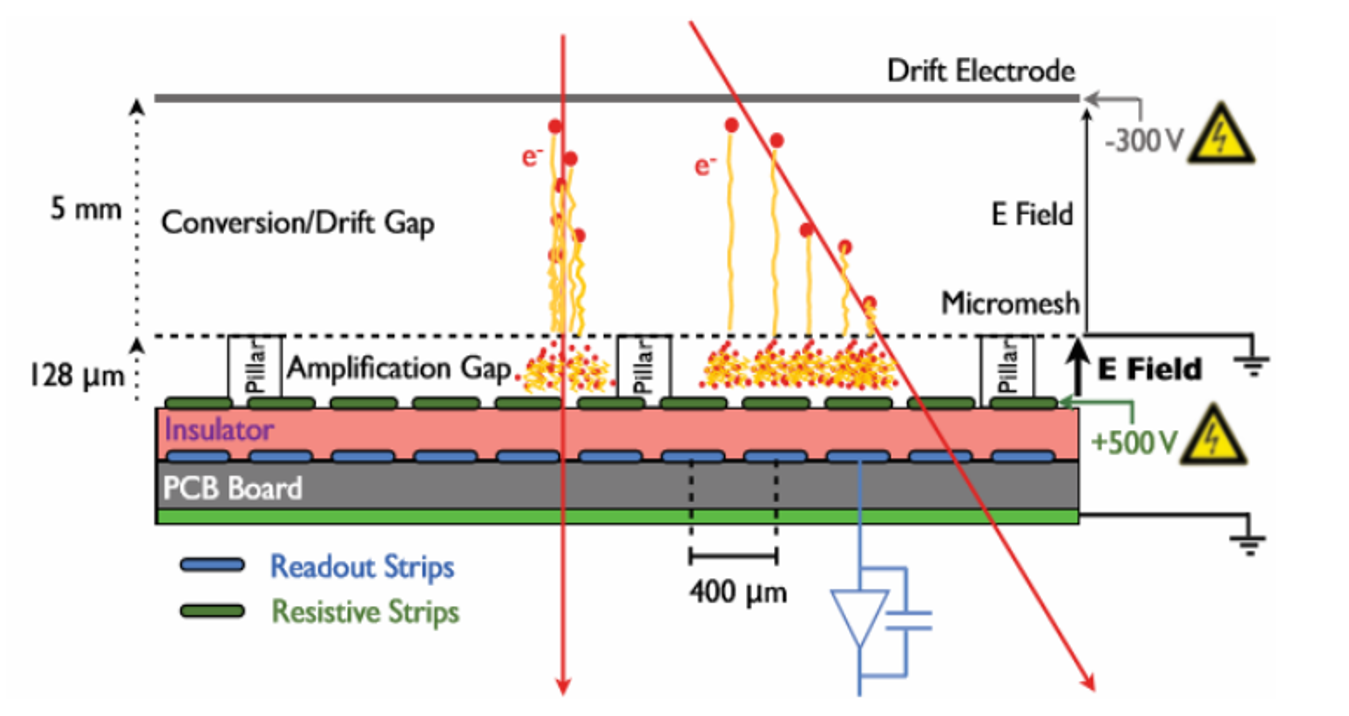
\includegraphics[width=0.4\textwidth]{schema_micromegas.png}
    \caption{Schema concettuale di una "bulk micromegas". Le dimensioni del gap di amplificazione ed i valori di tensione sono ottimizzati per la rivelazione di muoni di alta energia.}
    \label{fisica_micromegas}
\end{figure}
